\documentclass[10pt,a4paper]{scrreprt}
\usepackage[latin1]{inputenc}
\usepackage{graphicx}
\usepackage{float}
\usepackage{minted}
\usepackage[titletoc]{appendix}
\usepackage[margin=1in]{geometry}
\usepackage[hidelinks]{hyperref}
\usepackage{xcolor}
\definecolor{link}{rgb}{.2,.2,.2}
\definecolor{url}{rgb}{.1,.1,.6}
\hypersetup{
colorlinks=true,
linkcolor={link},
urlcolor={url}
}
\author{Kory Prince}
\title{The Movie Database}
\subtitle{User Documentation}
\date{}
\begin{document}
\maketitle
\tableofcontents

\chapter{Introduction}
The goal with this project was to create a very usable web frontend to a movie database. To make the project interesting, a lot of data was used, with the idea being that as much as possible it be based on fact. Movie data (on 860 movies) was pulled from The \href{http://www.themoviedb.org/}{Movie Database (TMDB)}. Reviewers were generated using \href{http://listofrandomnames.com/}{List of Random Names}. All ratings are based around the real user rating for each movie (as given by TMDB). In some cases there was no rating in which cases ratings defaulted to 0. All ratings are (re)generated when the application starts.

All data (except for the movie poster images which are stored on TMDB's servers) is stored in a \href{http://www.sqlite.org/}{SQLite3} database. A \href{http://www.python.org/}{Python} \href{http://uwsgi-docs.readthedocs.org/en/latest/}{uWSGI} application running behind \href{http://wiki.nginx.org/Main}{nginx} serves as a Web Frontend to the data. This application written entirely from scratch, uses custom templates and url mapping system to serve dynamic content to the end user.

The interface is fully \href{http://en.wikipedia.org/wiki/Responsive_web_design}{Responsive} and \href{http://en.wikipedia.org/wiki/Progressive_enhancement}{Progressive}. This means that the website can be viewed on older or more restrictive browsers and still work. The site will use features of the browser if present to enhance the experience (Use \href{http://www.mozilla.org/en-US/firefox/fx/#desktop}{Firefox} or \href{http://www.google.com/chrome/}{Chrome}.) Supports all major browsers (only IE8+. Please, let old IEs die a peaceful death.) Finally, the site scales down on mobile web browsers without sacrificing the content.

All code is given to the Public Domain where possible. TMDB data belongs to that organization.

\chapter{Installing the Application}
The Movie Database is a Python application running on uWSGI. Nginx is the webserver we use to interface with a user's browser. Ubuntu Linux is the server OS. This section will guide you on installing each of these components.

\section{Ubuntu}
This guide will not cover how to install Ubuntu Server, but it is fairly straightforward, and many guides can be found on the internet. We used Ubuntu 12.04. You can use this OS that supports python 2.7 and uWSGI.

\section{The Movie Database Code}
The source of The Movie Database is hosted on Github. You can download your own copy by using the following commands:

\begin{minted}{bash}
user@server:~$ sudo apt-get install unzip #needed for later command
user@server:~$ cd /tmp
user@server:/tmp$ wget https://github.com/korylprince/schoolprojects/archive/master.zip
user@server:/tmp$ unzip master.zip
user@server:/tmp$ sudo cp -R /tmp/schoolprojects-master/moviedb /opt/
\end{minted}

This will install the software in the /opt directory of your server.

\section{Movie Data}
The movie data must be generated as redistribution of the data is not permitted. You must obtain an API key from TMDB. Once the key is obtained you can edit the scrape.py file and use it to generate the data.

\begin{minted}{bash}
user@server:~$ cd /tmp/schoolprojects-master/moviedb/gen
user@server:/tmp/schoolprojects-master/moviedb/gen$ vim scrape.py #insert your api key!
\end{minted}

Next you must obtain the pytmdb3 library:

\begin{minted}{bash}
user@server:/tmp/schoolprojects-master/moviedb/gen$ wget \
> https://github.com/wagnerrp/pytmdb3/archive/master.zip
user@server:/tmp/schoolprojects-master/moviedb/gen$ unzip master.zip
user@server:/tmp/schoolprojects-master/moviedb/gen$ mv pytmdb3-master/tmdb3/ ./
\end{minted}

Finally we can run the scrape.py file:

\begin{minted}{bash}
user@server:/tmp/schoolprojects-master/moviedb/gen$ python scrape.py
\end{minted}

This last command can take a very long time because it will pull data from TMDB's servers. It can also consume large amounts of memory. Once done it will produce a movies file in the current directory. You will need to copy this to the application directory:

\begin{minted}{bash}
user@server:/tmp/schoolprojects-master/moviedb/gen$ sudo cp movies /opt/moviedb/gen/
\end{minted}

Finally, we must change the permissions of the application to the web server user:

\begin{minted}{bash}
user@server:~$ sudo chown -R www-data:www-data /opt/moviedb
\end{minted}

\section{uWSGI}
uWSGI can be installed from Ubuntu's package manager using terminal:
\begin{minted}{bash}
user@server:~$ sudo apt-get install uwsgi uwsgi-plugin-python
\end{minted}

Now we must create a configuration for our application:

\begin{minted}{bash}
user@server:~$ sudo vim /etc/uwsgi/apps-available/moviedb.ini
\end{minted}

In this file paste the following:

\begin{minted}{ini}
[uwsgi]
pythonpath = /opt/moviedb
chdir = /opt/moviedb
module = web                                                                    
processes = 1 
\end{minted}

Now we must enable the application and restart the service:

\begin{minted}{bash}
user@server:~$ sudo ln /etc/uwsgi/apps-available/moviedb.ini \
> /etc/uwsgi/apps-enabled/moviedb.ini
user@server:~$ sudo service uwsgi restart
\end{minted}

\section{Nginx}
Nginx is the webserver that will sit between the user's browser and uWSGI. You can use other web servers, but Nginx is very efficient and easy to configure. First to install nginx:

\begin{minted}{bash}
user@server:~$ sudo apt-get install nginx
\end{minted}

Now we must configure it:

\begin{minted}{bash}
user@server:~$ sudo vim /etc/nginx/sites-available/default
\end{minted}

Paste the following code:

\begin{minted}{nginx}
server {
    listen 80; 
    server_name movies.unstac.tk;
    root /opt/moviedb;

    charset utf-8;

    // robots.txt for no indexing
    location /robots.txt {
        try_files /static/robots.txt =404;
    }   

    location /static {
        try_files $uri $uri/ =404;
    }   

    location / { 
        uwsgi_pass unix:///run/uwsgi/app/moviedb/socket;
        include uwsgi_params;
    }   

    location ~ (.*.py|.*.pyc|.*.git.*) {
        return 404;
    }   
}
\end{minted}

Of course you must change movies.unstac.tk to your own server name.

Now just restart the server:

\begin{minted}{bash}
user@server:~$ sudo service nginx restart
\end{minted}

You should now be able to browse to your website and view it.

\chapter{Using the Application}
You can view a live application at \href{http://movies.unstac.tk/}{movies.unstac.tk} if you don't wish to install your own application.

\section{Home}
Upon visiting the web page, you will be presented with a page much like Figure 3.1. This page contains a Search box and the information found in the Introduction of this document.

\begin{figure}[H]
\centering
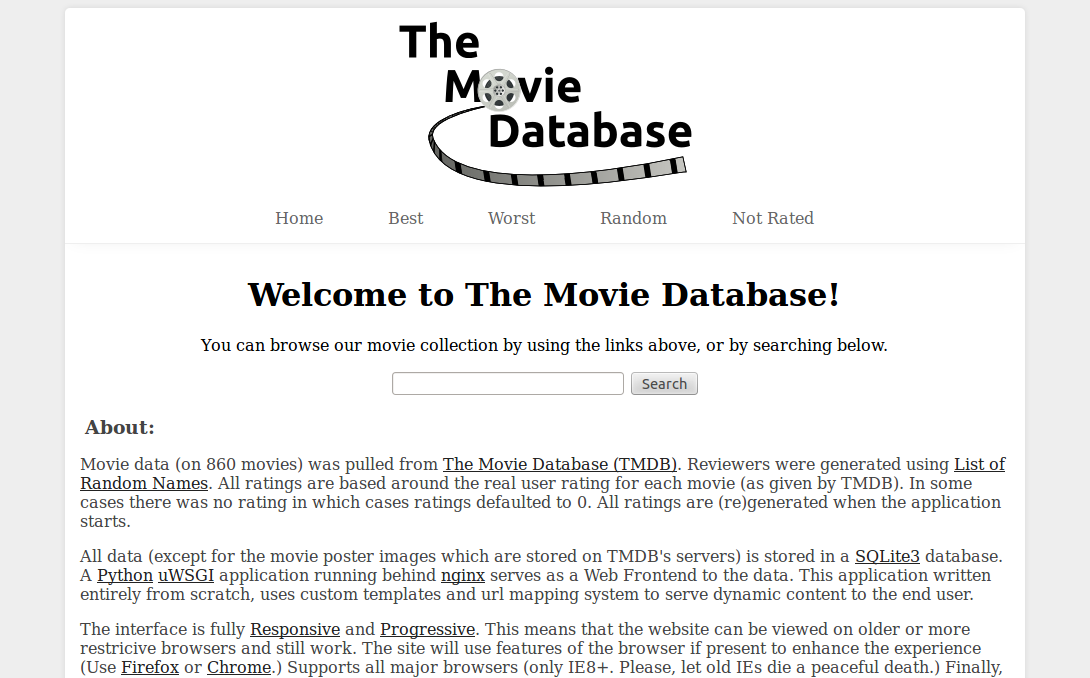
\includegraphics[scale=.25]{index.png}
\caption{Home page}
\end{figure}

\subsection{Navigation Bar}
The links along the top are present throughout the application. Clicking on Home or clicking the logo will take you to the current index page. Clicking Best, Worst, Random, or Not Rated will bring you to those respective pages.

\section{Best and Worst}
Clicking on Best or Worst will show a page much like Figure 3.2. The 10 Best or Worst movies will be shown.

\begin{figure}[H]
\centering
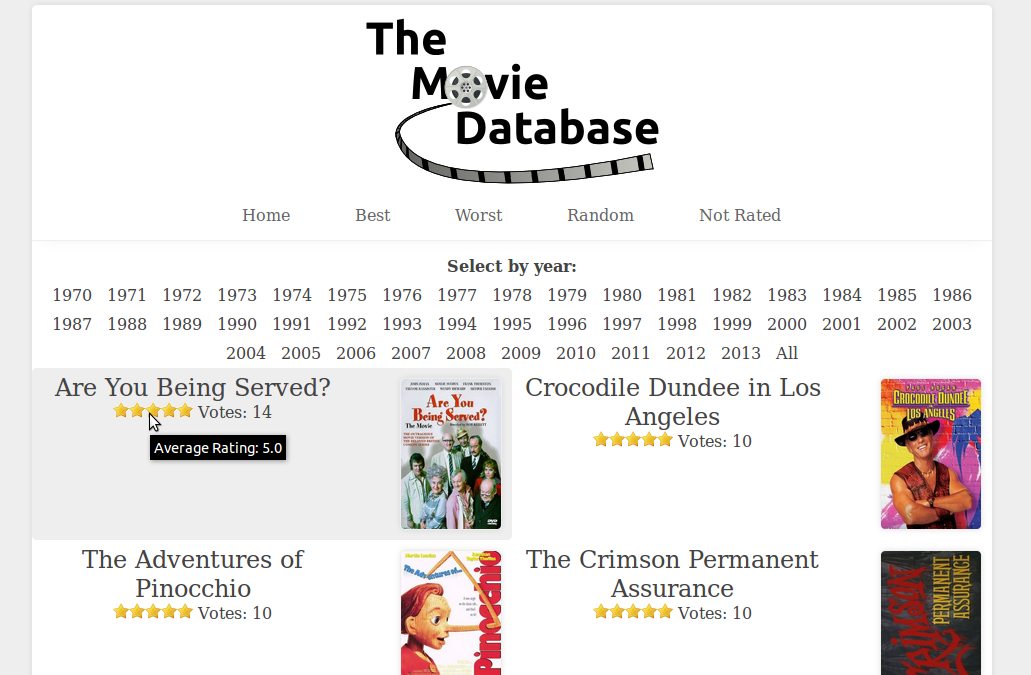
\includegraphics[scale=.25]{best.png}
\caption{Best page}
\end{figure}

\subsection{Year List}
You will see directly below the Navigation Bar there is a list of years. Each year that a movie in the database was produced in is listed here. Clicking on the year will bring you to the list of the 10 Best of Worst movies for that year. When showing a year, the year is listed like in Figure 3.3.

\begin{figure}[H]
\centering
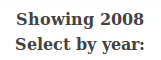
\includegraphics[scale=.5]{year.png}
\caption{Showing the selected year}
\end{figure}

\subsection{Movie List}
You will see that for each movie, the title, star rating, and movie poster will be shown. As shown in Figure 3.2, hovering over the stars will give a more exact average. Clicking on either the title of a movie will bring you to that movie's Movie Page.

\section{Random}
The Random page looks much like the Best or Worse page. The only differences are that each time the page is loaded, 10 different movies will appear, and the Year List will does not show on this page.

\section{Not Rated}
The Not Rated page will show any movies that have no ratings. This is the first page you might notice something different at the bottom of the screen, the Pager.

\section{Pager}
As you can see in Figure 3.4, there is a Next $\rightarrow$ link. This link will take you to the next page of results. This will only show if there are more results than showing on the current page.

\begin{figure}[H]
\centering
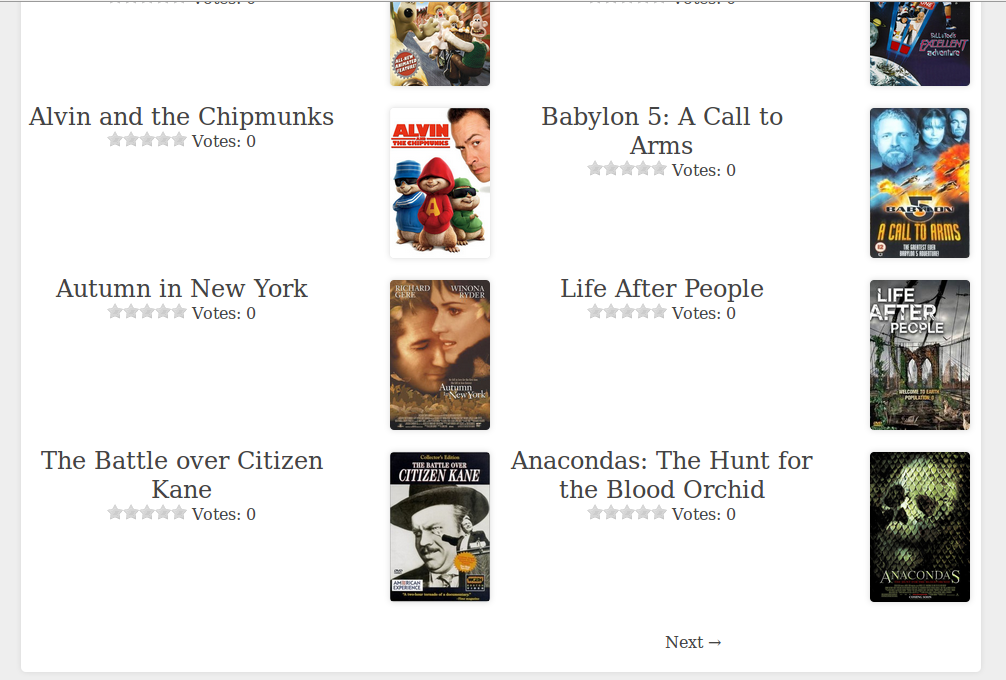
\includegraphics[scale=.25]{notrated.png}
\caption{The Next $\rightarrow$ link}
\end{figure}

If there are several pages you might see both the Next $\rightarrow$ link and the $\leftarrow$ Previous link as seen in Figure 3.5.

\begin{figure}[H]
\centering
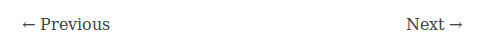
\includegraphics[scale=.5]{pager.png}
\caption{The full Pager}
\end{figure}

\section{Search}
As seen in Figure 3.1, the Home page contains a search box and button. Simply enter part or all of a movie title and click the Search button as shown in Figure 3.6.

\begin{figure}[H]
\centering

\includegraphics[scale=.5]{searchbox.png}
\caption{The Search box}
\end{figure}

If your query returns any results, they will be displayed in the same familiar list. If your search returns no results then you will see the page in Figure 3.7. Simply click the Home button or the link below to try another search.

\begin{figure}[H]
\centering
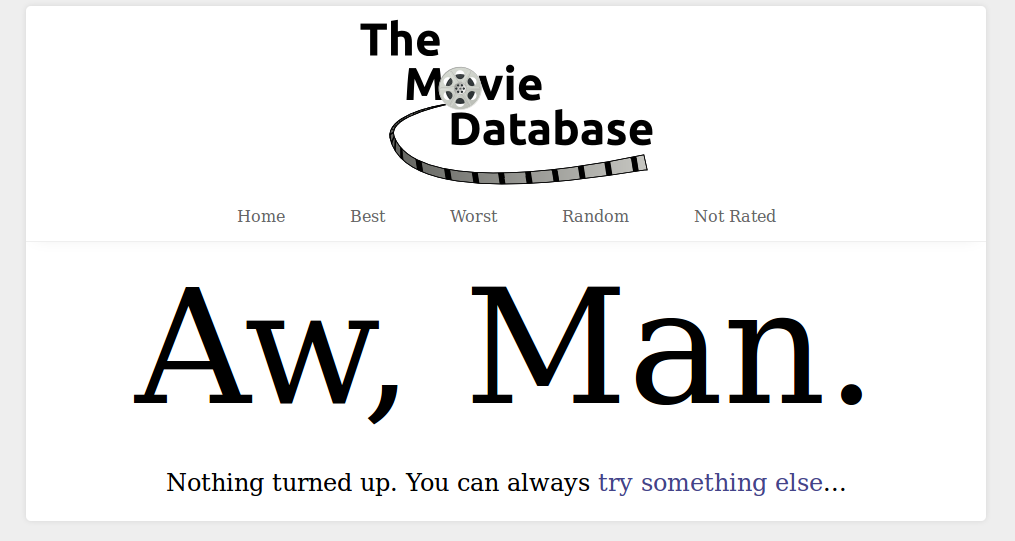
\includegraphics[scale=.25]{nosearch.png}
\caption{No results found}
\end{figure}

\section{Movie Page}
If you click on the poster or title of any movie in a Movie List, you will be taken to the Movie Page. As you can see in Figure 3.8, the Movie Page displays more information about the movie: The title, director, release year, average rating, a summary, and a larger version of the poster. Below this you can see some of the reviewers and the ratings they gave this movie. Clicking on the reviewer's avatar or name will bring you to that reviewer's Reviewer Page.

\begin{figure}[H]
\centering
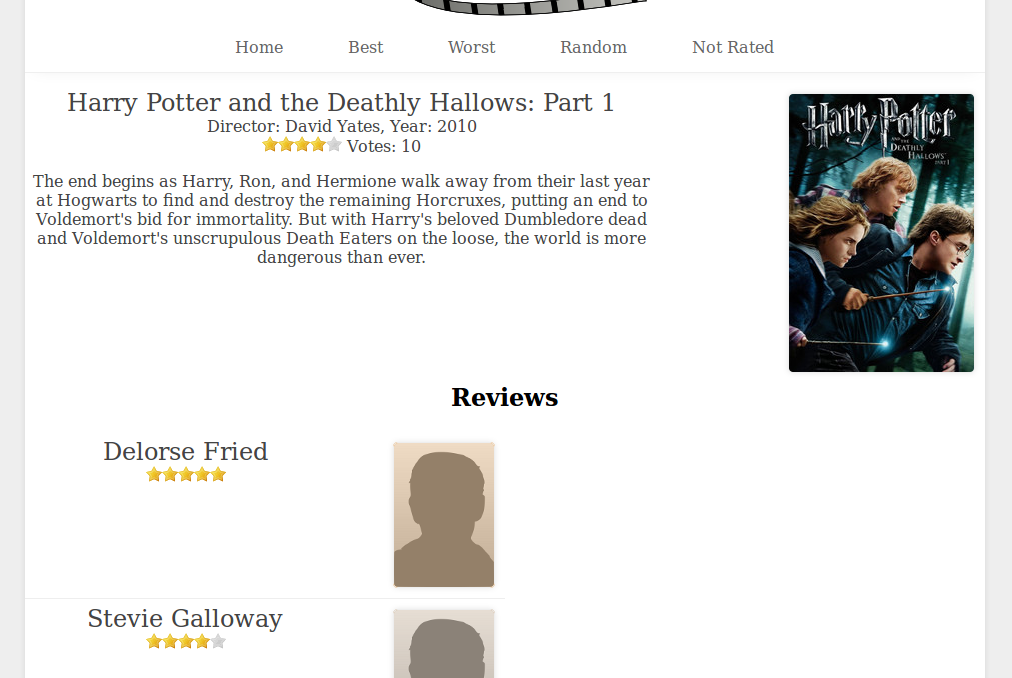
\includegraphics[scale=.25]{movie.png}
\caption{Movie Page}
\end{figure}

At the bottom of the screen you will see the Click to show all Reviews link as in Figure 3.9. Clicking on this link will show all reviews for the movie.

\begin{figure}[H]
\centering

\includegraphics[scale=.5]{showreviews.png}
\caption{Show all Reviews}
\end{figure}

\section{Reviewer Page}
Clicking on a reviewer's avatar or name will bring you to their Reviewer Page as show in Figure 3.10. This page is similar to the Movie Page. It will show the reviewer's avatar, average rating given, and number of votes. Below this is a list of movies reviewed by the reviewer and another Click to show all Reviews link that will show all movies reviewed by the reviewer.

\begin{figure}[H]
\centering
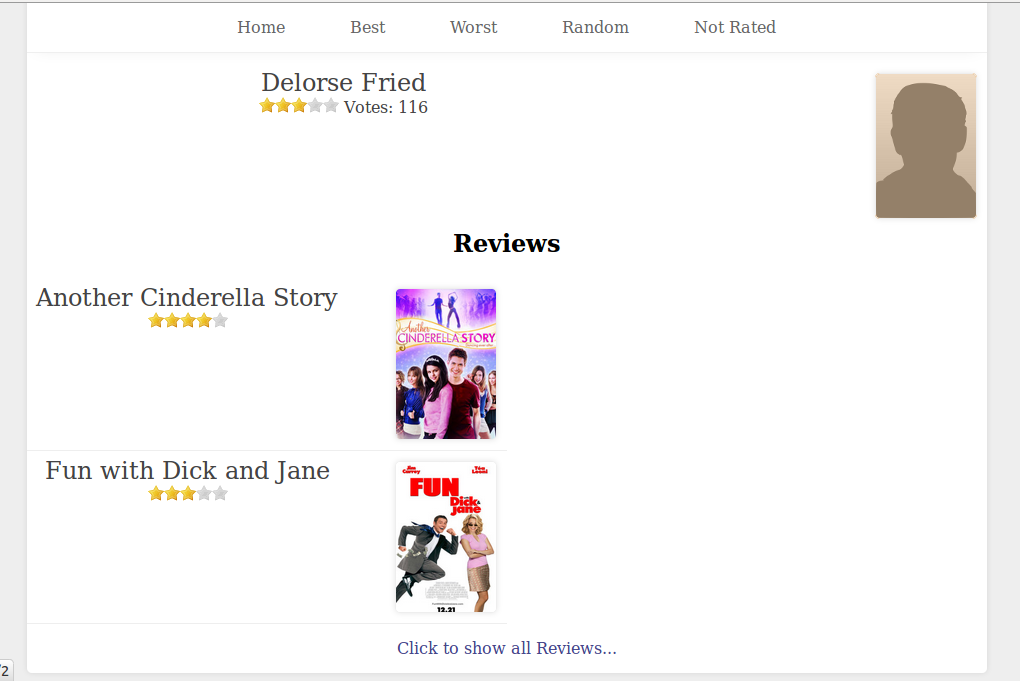
\includegraphics[scale=.25]{reviewer.png}
\caption{Reviewer Page}
\end{figure}

\chapter{Mobile Interface}
There is no separate Mobile Interface. Rather the application will transform its content to make better use of a smaller screen size. The application uses \href{http://www.w3.org/TR/css3-mediaqueries/}{CSS media queries} to scale the content to size, and some Javascript code to make some elements more usable on a smaller interface. If you would like to try out the Mobile Interface and see the content scale down in real time, you can use Firefox's Responsive Design View which comes with recent versions. Simply press CTRL+Shift+M to activate this feature. You can drag the corner handle of the web page to scale the page to any size and see how the application responds in real-time.

\section{Menu}
The Menu will collapse down to a single button on smaller screens. Clicking on the Menu button will show the Navigation links as seen in Figure 4.1.

\begin{figure}[H]
\centering
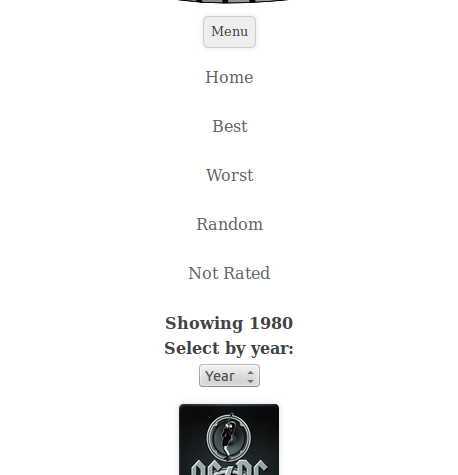
\includegraphics[scale=.5]{menu.png}
\caption{Mobile Menu}
\end{figure}

\section{Year List}
The Year List is far too big to show on smaller screens, so it is collapsed into a select box as shown in Figure 4.2. Selecting any year will bring you to that year's page.

\begin{figure}[H]
\centering
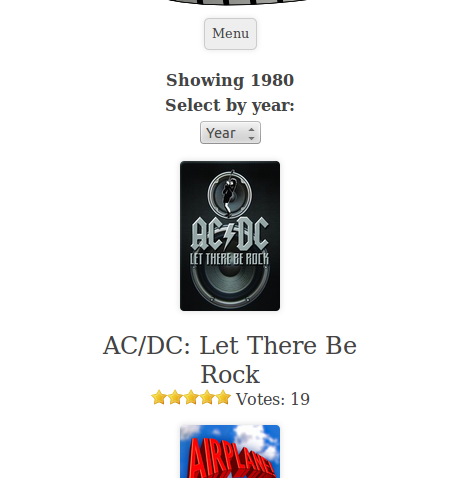
\includegraphics[scale=.5]{mobile.png}
\caption{Mobile Year List}
\end{figure}

\section{Movie List}
As seen in Figure 4.2, the Movie list is now only one movie wide, and has collapsed down to better facilitate smaller screens.

\section{Movie and Reviewer Page}
As seen in Figure 4.3, the Movie and Reviewer pages also collapse down to fit better on smaller screens.

\begin{figure}[H]
\centering

\includegraphics[scale=.5]{mobilemovie.png}
\caption{Mobile Movie Page}
\end{figure}

\begin{appendices}
\chapter{Source Code}
The following is are the source code for the entire application, except for the movie data which must be generated and the name list which can be obtained from the Github repository.

\section{SQL Files}
\subsection{create.sql}

\begin{minted}{sql}
create table movie (
    movieID integer primary key autoincrement,
    title varchar(100),
    director varchar(50),
    year decimal(4,0),
    poster varchar(100), /* Extra field for movie poster */
    overview text /* Extra Field for movie description */
);

create table reviewer (
    reviewerID integer primary key autoincrement,
    name varchar(50)
);

create table rating (
    movieID integer,
    reviewerID integer,
    ratingDate date,
    stars integer,
    primary key (movieID,reviewerID), /* While the relation is many to many,
        no reviewer will review a movie twice. Besides,
        I'm generating the data so I know this holds. */
    foreign key (movieID) references movie (movieID),
    foreign key (reviewerID) references reviewer (reviewerID)
);
\end{minted}

\subsection{drop.sql}

\begin{minted}{sql}
drop table rating;
drop table movie;
drop table reviewer;
\end{minted}

\section{Python}
\subsection{scrape.py}

\begin{minted}{python}
import tmdb3 as t # uses https://github.com/wagnerrp/pytmdb3
import pickle
import sys

t.set_key('YOUR API KEY')
b = t.searchMovie('a')
movies = []
for y in range(len(b)):
    try:
        sys.stdout.write(str(y)+',')
        x = b[y]
        # we want recent movies
        if x.releasedate.year < 1970:
            continue
        # and movies in English
        if 'English' not in [y.name for y in x.languages]:
            continue
        # and decent movies
        if x.releases['US'].certification not in [u'G',u'PG',u'PG-13']:
            continue
        movie = dict()
        movie['title'] = x.title
        movie['year'] = x.releasedate.year
        movie['date'] = x.releasedate
        movie['director'] = [y.name for y in x.crew if 
                y.job == 'Director'][0] or 'Director Unknown'
        movie['poster'] = x.poster.geturl('w185')
        movie['rating'] = x.userrating
        movie['overview'] = x.overview
        movies.append(movie)
        print len(movies)
    except KeyboardInterrupt:
        break
    except:
        print 'Error on: ',x
    if len(movies) == 2500:
        break

#dump to pickle file
with open('movies','w') as f:
    pickle.dump(movies,f)

\end{minted}

\subsection{db.py.py}

\begin{minted}{python}
import sqlite3
import db
import re
import urlparse

def application(env, start_response):
    #main handler called every request
    url = env['PATH_INFO']
    content = mapper(url,env,start_response)
    # if not returning normally, let function handle output
    if content is None:
        return
    # otherwise put everything in the template
    return templates['main'].format(**content).encode('utf-8')

def mapper(url,env,start_response):
#maps given urls to functions
    #remove trailing /
    if url[-1] == '/' and len(url) != 1:
        url = url[:-1]
    parsed = url_match.match(url)
    if parsed is None or parsed.groupdict() is None:
        return url_404(start_response)
    else:
        # reassemble url and check in map
        params = parsed.groupdict()
        paramlist = [x for x in [params['func'],'#' 
            if params['num'] else None,params['sub']] if x is not None]
        url = '/'+'/'.join(paramlist)
        if url in path_map:
            # call function with parameters
            func = path_map[url][:] #use copy
            if '#' in func:
                func[func.index('#')] = int(params['num'])
            if 'get' in func:
                func[func.index('get')] = urlparse.parse_qs(env['QUERY_STRING'])
            response, content = func[0](*func[1:])
            start_response(*response)
            return content 
        else:
            return url_404(start_response)

##
## url functions
##

def url_404(start_response):
    start_response('404 Not Found', [('Content-Type','text/html')])
    return {'title':u'Oops','content':templates['not_found']}

def url_index():
#/ -> index with search, links, and featured movies (3 highest rated)
    return (('200 OK', [('Content-Type','text/html')]),
        {u'title':u'Welcome','content':templates['index']})

def url_best(year=False):
#/best -> 10 best of all time
#/best/<year> -> 10 best of year
    out = ['{0}<h4>Select by year:</h4><span class="yearwrapper">'.format(
    '<h4>Showing {0}</h4>'.format(year) if year else ''
    )]
    for y in db.get_years(conn):
        out.append('<a href="/best/{0}">{0}</a> '.format(y))
    out.append('<a href="/best">All</a></span>')
    movielist = movie_list_gen(db.get_best_worst(conn,'desc',year))
    if movielist == []:
        return (('404 Not Found', [('Content-Type','text/html')]),
            {'title':u'Oops','content':templates['not_found']})
    out += movielist
    return (('200 OK', [('Content-Type','text/html')]),
        {'title':u'Best Movies of ' 
        + (unicode(year) if year else u'All Time'),'content':u''.join(out)})

def url_worst(year=False):
#/worst -> 10 worst of all time
#/worst/<year> -> 10 worst of year
    out = ['{0}<h4>Select by year:</h4><span class="yearwrapper">'.format(
    '<h4>Showing {0}</h4>'.format(year) if year else ''
    )]
    for y in db.get_years(conn):
        out.append('<a href="/worst/{0}">{0}</a> '.format(y))
    out.append('<a href="/worst">All</a></span>')
    movielist = movie_list_gen(db.get_best_worst(conn,'asc',year))
    if movielist == []:
        return (('404 Not Found', [('Content-Type','text/html')]),
                {'title':u'Oops','content':templates['not_found']})
    out += movielist
    return (('200 OK', [('Content-Type','text/html')]),
        {'title':u'Worst Movies of '
        + (unicode(year) if year else u'All Time'),'content':u''.join(out)})

def url_random():
#/random -> 10 random movies
    out = movie_list_gen(db.get_random(conn))
    return (('200 OK', [('Content-Type','text/html')]),
        {'title':u'Random','content':u''.join(out)})

def url_none(page):
#/none/<page> -> movies with no rating with paging
    rows = db.get_none(conn,page)
    flags = []
    out = movie_list_gen(rows,flags)
    if out == []:
        return (('404 Not Found', [('Content-Type','text/html')]),
            {'title':u'Oops','content':templates['not_found']})
    out.append(pager_gen('none',page,'more' in flags))
    return (('200 OK', [('Content-Type','text/html')]),
        {'title':u'Not Rated','content':u''.join(out)})

def url_search(query,page):
#/search/<num> -> search based on post data with paging
    try:
        search = query['s'][0]
        rows = db.get_search(conn,page,search)
    except KeyError, IndexError:
        return (('400 Bad Request', [('Content-Type','text/html')]),
            {'title':u'Oops','content':templates['bad_request']})
    flags = []
    out = movie_list_gen(rows,flags)
    if out == []:
        out = ['<span class="error">Aw, Man.</span><p class="error_text">\
            Nothing turned up. You can always <a href="/">\
            try something else</a>...</p>']
    else:
        out.append(pager_gen('search',page,'more' in flags,'?s='+search))
    return (('200 OK', [('Content-Type','text/html')]),
            {'title':u'Searching: '+search,'content':u''.join(out)})

def url_movie(movieID):
#/movie/<num> -> movie page
    row = db.get_movie(conn,movieID)
    if row is None:
        return (('404 Not Found', [('Content-Type','text/html')]),
            {'title':u'Oops','content':templates['not_found']})
    row = dict(row)
    row['stars'] = star_gen(row['stars'],row['votes'])
    row['reviews'] = reviewer_list_slim_gen(db.get_reviews_by_movie(conn,movieID))
    out = templates['movie_full'].format(**row)
    return (('200 OK', [('Content-Type','text/html')]),
        {'title':row['title'],'content':out})

def url_reviewer(reviewerID):
#/reviewer/<num> -> reviewer page
    row = db.get_reviewer(conn,reviewerID)
    if row is None:
        return (('404 Not Found', [('Content-Type','text/html')]),
            {'title':u'Oops','content':templates['not_found']})
    row = dict(row)
    row['stars'] = star_gen(row['stars'],row['votes'])
    row['color'] = color_gen(row['name'])
    row['reviews'] = movie_list_slim_gen(db.get_reviews_by_reviewer(conn,reviewerID))
    out = templates['reviewer_full'].format(**row)
    return (('200 OK', [('Content-Type','text/html')]),
        {'title':row['name'],'content':out})

def url_redirect(url):
    return (('302 Found', [('Location',url),('Content-Type','text/html')]),None)

##
##  Helper Functions
##

def movie_list_gen(cursor,flags = None):
#generate list of movies
    out = []
    count = 0
    for row in cursor:
        # check if there's another page
        if count >= 10:
            if flags is not None:
                flags.append('more')
            return out
        count += 1
        row = dict(row)
        row['stars'] = star_gen(row['stars'],row['votes'])
        out.append(templates['movie_brief'].format(**row))
    return out

def movie_list_slim_gen(cursor):
#generate list of reviews
    out = []
    for row in cursor:
        row = dict(row)
        row['stars'] = star_gen_single(row['stars'])
        out.append(templates['movie_slim'].format(**row))
    return u''.join(out)

def reviewer_list_slim_gen(cursor):
#generate list of reviews
    out = []
    for row in cursor:
        row = dict(row)
        row['stars'] = star_gen_single(row['stars'])
        row['color'] = color_gen(row['name'])
        out.append(templates['reviewer_slim'].format(**row))
    return u''.join(out)

def pager_gen(func,page,more,query=''):
# generates pager navigation
    out = ['<nav class="pager">']
    if page > 1:
        out.append('<a class="pager_left" href="/{0}/{1}{2}">&larr; Previous</a>'.format(
            func,page-1,query
        ))
    if more:
        out.append('<a class="pager_right" href="/{0}/{1}{2}">Next &rarr;</a>'.format(
            func,page+1,query
        ))
    out.append('</nav>')
    return u''.join(out)

def star_gen(rating, votes):
#generate star output based on rating and votes
    if rating is None:
        rating = 0
        votes = 0
    out = ['<div title="Average Rating: {0}">'.format(round(rating,2))]
    rating = int(round(rating))
    for star in range(5):
        if star < rating:
            out.append('<span class="star"></span>')
        else:
            out.append('<span class="nostar"></span>')
    out.append(' <span class="votes">Votes: {0}</span></div>'.format(votes))
    return u''.join(out)

def star_gen_single(rating):
#generate star output based on single rating 
    if rating is None:
        rating = 0
    out = ['<div>']
    rating = int(round(rating))
    for star in range(5):
        if star < rating:
            out.append('<span class="star"></span>')
        else:
            out.append('<span class="nostar"></span>')
    out.append('</div>')
    return u''.join(out)

def color_gen(name):
    #generates random color based on name
    c = hex(hash(name))
    if len(c) < 8:
        return '#'+c[2:]+'f'*(8-len(c))
    return '#' + c[-6:]

##
## Performed Every Restart
##
     
# connect to database and generate it
conn = sqlite3.connect('ratings.db')
conn.row_factory = sqlite3.Row
db.create(conn)

# read template files
templates = {}
with open('templates/main.html') as f:
    templates['main'] = unicode(f.read())
with open('templates/index.html') as f:
    templates['index'] = unicode(f.read())
with open('templates/movie_full.html') as f:
    templates['movie_full'] = unicode(f.read())
with open('templates/movie_brief.html') as f:
    templates['movie_brief'] = unicode(f.read())
with open('templates/movie_slim.html') as f:
    templates['movie_slim'] = unicode(f.read())
with open('templates/reviewer_full.html') as f:
    templates['reviewer_full'] = unicode(f.read())
with open('templates/reviewer_slim.html') as f:
    templates['reviewer_slim'] = unicode(f.read())
with open('templates/400.html') as f:
    templates['bad_request'] = unicode(f.read())
with open('templates/404.html') as f:
    templates['not_found'] = unicode(f.read())

# define urls
path_map = {
    '/' : [url_index],
    '/best' : [url_best],
    '/best/#' : [url_best,'#'],
    '/worst' : [url_worst],
    '/worst/#' : [url_worst,'#'],
    '/random' : [url_random],
    '/none' : [url_redirect,'/none/1'],
    '/none/#' : [url_none,'#'],
    '/search' : [url_redirect,'/'],
    '/search/#' : [url_search,'get','#'],
    '/movie' : [url_redirect,'/'],
    '/movie/#' : [url_movie,'#'],
    '/reviewer' : [url_redirect,'/'],
    '/reviewer/#' : [url_reviewer,'#']
}

#compile regex
url_match = re.compile("/(?:(?P<func>[a-z]+)(?:/(?P<num>[1-9][0-9]*)(?:/(?P<sub>[a-z]+))?)?)?$")
\end{minted}

\section{Style}
\subsection{style.css}

\begin{minted}{css}
body {
    background-color: #eee;
    text-align: center;
}

a,img {
    border: none; /* remove ugly IE border */
}

#logo {
    max-width: 100%;
    width: auto;
    padding-top: 10px;
    border: none;
}

#mainwrapper {
    width: 100%;
    max-width: 960px;
    background-color: #fff;
    margin-left: auto;
    margin-right: auto;
    -webkit-border-radius: 5px;
    -moz-border-radius: 5px;
    border-radius: 5px;
    -webkit-box-shadow: 0px 0px 5px 0px rgba(0, 0, 0, .1);
    box-shadow: 0px 0px 5px 0px rgba(0, 0, 0, .1); 
    overflow: hidden;
}

#main-navigation {
    -webkit-box-shadow: 0px 5px 15px -10px rgba(0, 0, 0, .1);
    box-shadow: 0px 5px 15px -10px rgba(0, 0, 0, .1); 
    border-bottom: 1px solid #efefef;
    margin-bottom: 10px;
}

#main-navigation ul {
    margin: 0px;
    padding: 0px;
}

.nav-item {
    display: inline-block;
    padding: 15px 30px;
    -webkit-border-radius: 5px;
    -moz-border-radius: 5px;
    border-radius: 5px;
}

.nav-item:hover {
    background-color: #fcfcfc;
} 
.nav-item a {
    color: #666;
    text-decoration: none;
}

.nav-item:hover a {
    color: #222;
}

#content {
    overflow: hidden;
}

h3,h4 {
    margin: 5px;
    color: #444;
}

.left {
    text-align: left;
    padding: 15px;
    color: #444;
}

.left a {
    color: #222;
}

.left a:hover {
    color: #008;
}

.yearwrapper {
    width: 100%;
    clear: both;
    display: block;
}

.yearwrapper a {
    display: inline-block;
    padding: 5px;
    color: #444;
    text-decoration: none;
}

.yearwrapper a:hover {
    color: #222;
    text-decoration: underline;
}

.movie_brief {
    width: 50%;
    float: left;
    display: inline-block;
    -webkit-border-radius: 5px;
    -moz-border-radius: 5px;
    border-radius: 5px;
}

.movie_brief:hover {
    background-color: #eee;
}

.movie_meta {
    float: left;
    margin: 5px;
    width: 65%;
    color: #444;
}

.movie_title {
    font-size: 1.5em;
    text-decoration: none;
    color: #444;
}

.movie_title:hover {
    color: #222;
}

.movie_poster {
    float: right;
    margin: 10px;
    border: 1px solid #eee;
    -webkit-border-radius: 5px;
    -moz-border-radius: 5px;
    border-radius: 5px;
    line-height: 0;
    -webkit-box-shadow: 0px 0px 5px 0px rgba(0, 0, 0, .1);
    box-shadow: 0px 0px 5px 0px rgba(0, 0, 0, .1); 
    overflow:hidden;
}

.movie_poster:hover {
    -webkit-box-shadow: 0px 0px 5px 0px rgba(0, 0, 0, .3);
    box-shadow: 0px 0px 5px 0px rgba(0, 0, 0, .3); 
}

.movie_brief img, .movie_slim img {
    height: 150px;
    width: 100px;
}

.avatar img {
    height: auto;
    width: auto;
    opacity:0.8;
    filter:alpha(opacity=80);
}

.movie_full h2 {
    clear: both;
}

.movie_slim {
    width: 50%;
    clear: both;
    overflow: hidden;
    border-bottom: 1px solid #eee;
}

.pager {
    width: 100%;
    max-width: 480px;
    clear: both;
    margin: auto;
}

.pager_left, .pager_right {
    float: left;
    padding: 20px;
    color: #444;
    text-decoration: none;
}

.pager_left:hover, .pager_right:hover {
    color: #222;
    text-decoration: underline;
}

.pager_right {
    float: right;
}

.star, .nostar {
    width: 16px;
    height: 16px;
    display: inline-block;
    padding: 0px;
    margin: 0px;
    background-image:url('stars.gif');
    background-repeat:no-repeat;
    background-position: center bottom;
}

.nostar {
    background-position: center top;
}

.error {
    font-size: 10em;
}

.error_text {
    font-size: 1.5em;
}

.error_text a, #showreviews {
    color: #448;
    text-decoration: none;
}

#showreviews {
    display: inline-block;
    margin: 15px;
}

.error_text a:hover, #showreviews:hover {
    color: #222;
    text-decoration: underline;
}

/* Downsize movie displays */
@media (max-width: 800px) {

    body {
        margin: 0px;
    }

    #mainwrapper {
        -webkit-border-radius: none;
        -moz-border-radius: none;
        border-radius: none;
        -webkit-box-shadow: none;
        box-shadow: none; 
    }

    .movie_brief, .movie_slim {
        width: 100%;
    }

    .movie_meta,.movie_poster {
        float: none;
        margin-left: auto;
        margin-right: auto;
    }

    .movie_poster {
        display: inline-block;
    }
}

/* Collapse Menu, downsize, and hide some elements */
@media (max-width: 640px) {

    #main-navigation { 
        -webkit-box-shadow: none;
        box-shadow: none; 
        border-bottom: none;
    }
    
    /* hide only if js is enabled */
    .js #main-navigation ul { 
        display: none;
    }

    .js .yearwrapper { 
        display: none;
    }
    
    .nav-item {
        display: block;
        margin: auto;
    }

    #menu_button {
        display: inline-block;
        padding: 7px;
        font-size: .8em;
        background-color: #eee;
        color: #444;
        border: 1px solid #ccc;
        -webkit-border-radius: 5px;
        -moz-border-radius: 5px;
        border-radius: 5px;
        -webkit-box-shadow: 0px 0px 5px 0px rgba(0, 0, 0, .1);
        box-shadow: 0px 0px 5px 0px rgba(0, 0, 0, .1); 
        margin-top: 5px;
        margin-bottom: 5px;
    }

    #menu_button:hover {
        background-color: #f4f4f4;
        color: #000;
    }

    #yearselector {
        margin-bottom: 5px;
    }

    .error {
        font-size: 6em;
    }

    .error_text {
        font-size: 2em;
    }
}
\end{minted}

\section{Javascript}
\subsection{responsive.js}

\begin{minted}{js}
$(document).ready(function() {
    function resize() {
        // if screen is small
        if(Modernizr.mq('(max-width:640px)')) {
            // Convert Menu to button
            if ( $("#menu_button").length == 0 ) {
                $("#main-navigation").prepend('<span id="menu_button" >Menu</span>');
                $("#main-navigation ul").hide();
            }
            //generate select menu
            if ( $(".yearwrapper").length == 1 ) {
                $(".yearwrapper").hide();

                if ( $("#yearselector").length == 0 ) {
                    $(".yearwrapper").before('<select id="yearselector"></select>');
                    $("#yearselector").append('<option value="">Year</option>');
                    $(".yearwrapper a").each(function(){
                        $("#yearselector").append(
                        '<option value="'+$(this).attr('href')+'">'+$(this).html()+'</option>'
                        );
                    });
                }
            } 
        }
        else {
            $("#menu_button").remove();
            $("#main-navigation ul").show()

            $(".yearwrapper").show();
            $("#yearselector").remove();
        }
    }

    // Add toggle behavior to button
    $("#main-navigation").on('click','#menu_button',function (e) {
        if ($("#main-navigation ul").css("display") == "none") {
            $("#main-navigation ul").show();
        }
        else {
            $("#main-navigation ul").hide();
        }
    });

    // Add link functionality to year selector
    $("#content").on("change","#yearselector",function(e) {
        if ($(this).val() != '') {
            window.location = $(this).val();
        }
    });

    // Call on resize, use timeout to buffer
    var timerID;
    $(window).resize(function() {
        clearTimeout(timerID);
        id = setTimeout(resize, 10);
    });
    resize();

    if ($(".reviews").length == 1 && $(".reviews").children().length > 2) {
        $(".reviews").children().slice(2).hide();
        $(".reviews").after('<a id="showreviews">Click to show all Reviews...</a>');
    }
    $("#content").on("click","#showreviews",function(e) {
        $(".reviews").children().show();
        $("#showreviews").hide();
    });
});
\end{minted}

\section{Templates}


\inputminted{html}{templates.html}

\end{appendices}
\end{document}